\documentclass{article}

% Environment setup

\usepackage[
    margin=.75in
]{geometry} %geometry (sets margin) and other useful packages 

\setlength{\parindent}{0em}
\setlength{\parskip}{.5em}

\usepackage{graphicx}
\usepackage{grffile}  % support extra dots in filenames
\usepackage{fancyref}
\usepackage[labelfont=bf]{caption}
\usepackage{subcaption}

\usepackage{chngcntr} \counterwithin{figure}{section}


\title{\textbf{CS 4641:} Unsupervised Learning and Dimensionality Reduction}
\author{Bradley Reardon}
\date{March 24, 2019}

\begin{document}
  \maketitle

  \section{Introduction}
    In this assignment, we are tasked with implementing two clustering algorithms and four dimensionality reduction algorithms, and seeing how they perform when applied both separately and together on two data sets. In addition, we'll take a focus on comparing these results to those of previous assignments when run on the same data sets. For comparison, all tests run for the purpose of this report will run each algorithm over 500 iterations, with a fixed seed to ensure reproducibility across tests.

    \subsubsection{Car data set}
      The Car Evaluation Database was created in June, 1997 by Marko Bohanec. It contains 1728 instances and 6 attributes. The purpose of this database is to attempt to classify a car as an unacceptable, acceptable, good, or very good choice based on factors including cost of ownership, comfort, and safety. Full details about the data set can be found at the source link below. Note that the instances of this data set completely cover the attribute space, making it an interesting problem for testing overfitting.

      \textbf{Source:} https://archive.ics.uci.edu/ml/datasets/car+evaluation

    \subsubsection{Breast Cancer Wisconsin data set}
      The Breast Cancer Wisconsin data set was donated to the UCI Machine Learning Repository in 1992, and contains data from one doctor's clinical cases, gathered from January 1989 to November 1991. In total, there are 699 instances signifying information about breast tumors such as clump thickness, uniformity in shape and size, and other screening factors. Data points are identified by two classes -- benign or malignant. The features of the data points are encoded as 9 continuous attributes rating the screening factor from 1 to 10.

      \textbf{Source:} https://archive.ics.uci.edu/ml/datasets/Breast+Cancer+Wisconsin+\%28Original\%29

  \section{Clustering}
    Clustering algorithms are a method for unsupervised learning which attempt to place a number of instances into clusters based on the closest mean of input attributes to an existing prototype. Because clustering would occur in either 6 or 9 dimensions, the main focus of analysis will be scoring the algorithms for each data set, though visualizations of these clusters do still show interesting information.

    \subsection{$k$-means Clustering}
      \subsubsection{Parameter selection}
        The main parameter for the $k$-means clustering algorithm is a value $k$, being the number of clusters that the algorithm will divide the data into. For both data sets, $k$ values of $2, 3, 4, 5, 6$ were tested for best performance. Each run of the algorithm used 20 initializations to ensure that the best possible cluster labeling is chosen for each data set. Smart initialization of clusters using the ``k-means++'' method ensure initial prototypes outperform random chance.

        The car data set did not perform very well in any of the $k$-means tests, with a maximum silhouette score of 0.119 being reported at a value of $k=3$. However, the data was known to be separated into 4 output classes, and the completeness of the instances over the attribute space led me to believe that a subset of the data may perform better.

        Running the algorithm again with only 500 of the 1728 total instances resulted in better silhouette scores overall, with the best performance occurring at $k=4$. \Fref{fig:km-silhouette-car} shows the silhouette plot and cluster visualization for this run.

        \begin{figure}[htb]
        \centering
        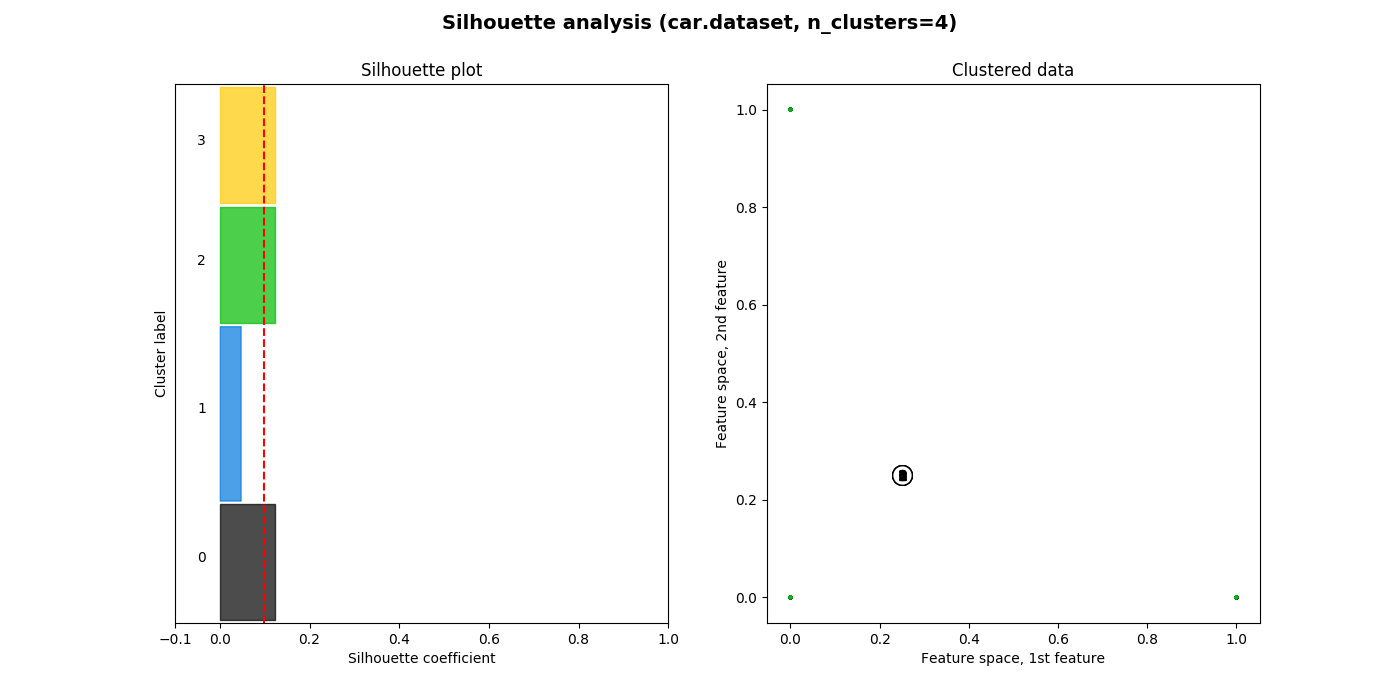
\includegraphics[width=\linewidth]{out/kmeans/car-4-clusters.png}
        \caption{Silhouette plot and clustered data visualization on two features for the car data set.}
        \label{fig:km-silhouette-car}
        \end{figure}

        The breast cancer data set was clustered better, with a best-performing $k=2$, matching the number of output classes. This resulted in a silhouette score of 0.577, which is much higher than that of the car data set. \Fref{fig:km-silhouette-cancer} shows the same visualizations for the cancer data set, which also reveals a very clear separation between the two clusters on the feature spaces for the first two features.

        \begin{figure}[htb]
        \centering
        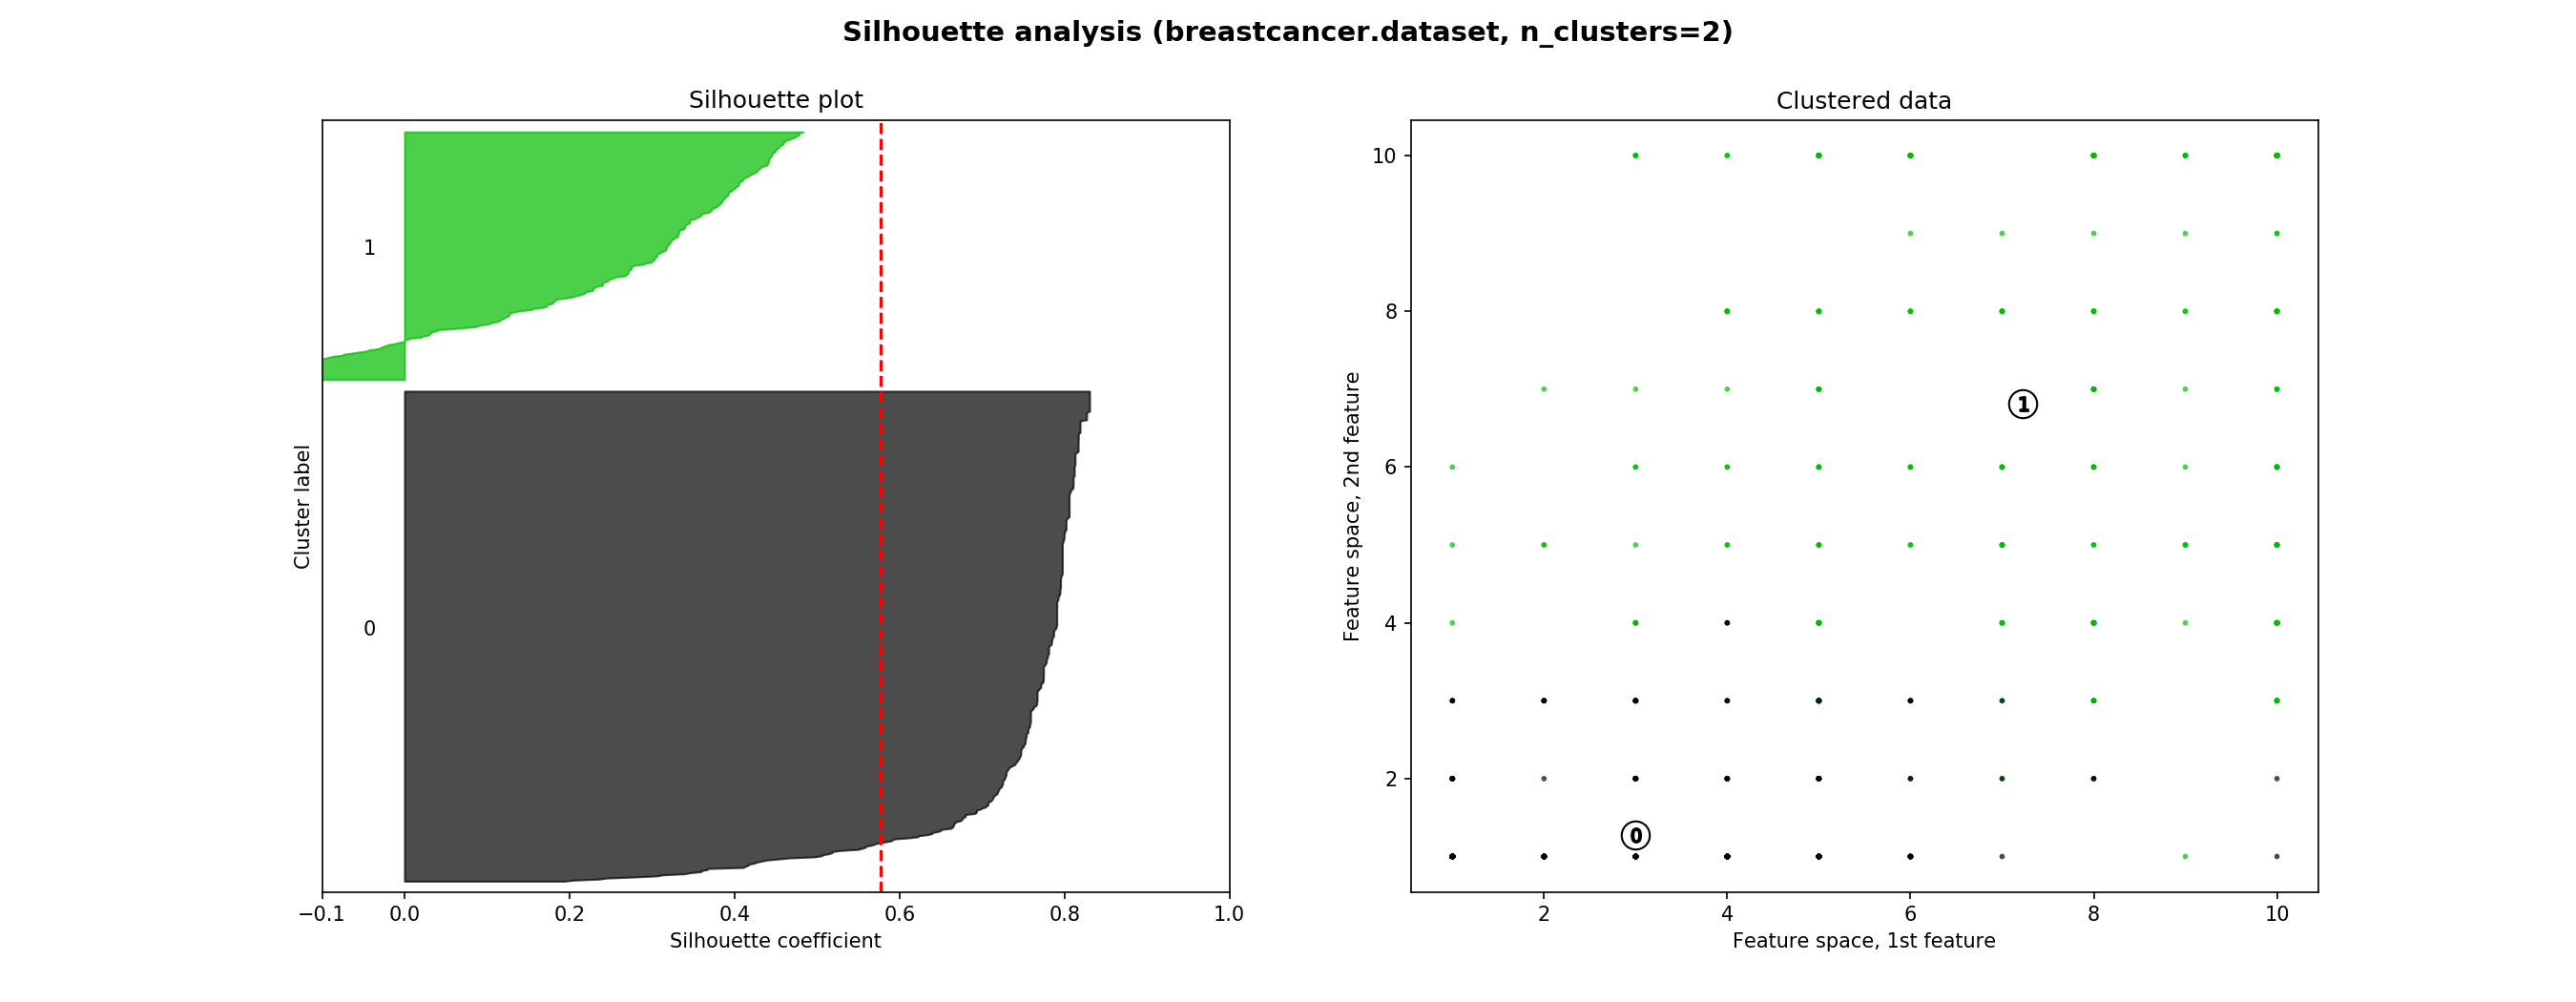
\includegraphics[width=\linewidth]{out/kmeans/cancer-2-clusters.png}
        \caption{Silhouette plot and clustered data visualization on two features for the cancer data set.}
        \label{fig:km-silhouette-cancer}
        \end{figure}

      \subsubsection{Performance}
        Using the ideal $k$ values of 4 and 2 for the cancer and car data sets respectively, learning curves were generated to evaluate the performance over the two data sets. These curves can be found in \Fref{fig:kmeans-learning}.

        \begin{figure}[htb]
        \centering

          \begin{subfigure}{0.5\textwidth}
            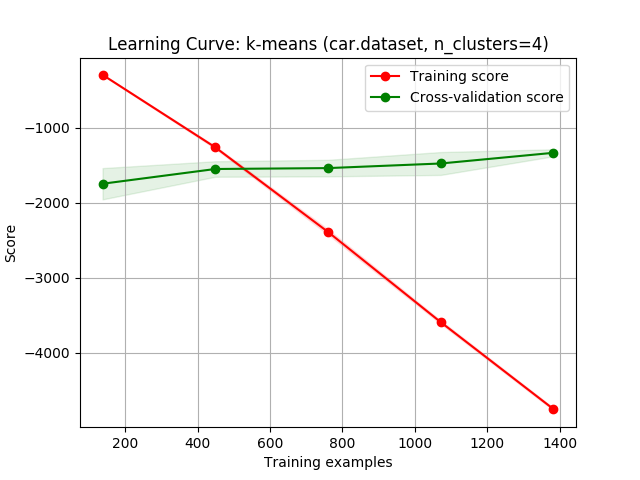
\includegraphics[width=\linewidth]{out/kmeans/car-learning.png}
            \caption{Learning curve, car.dataset}
            \label{fig:kmeans-learning-car}
          \end{subfigure}\hfil
          \begin{subfigure}{0.5\textwidth}
            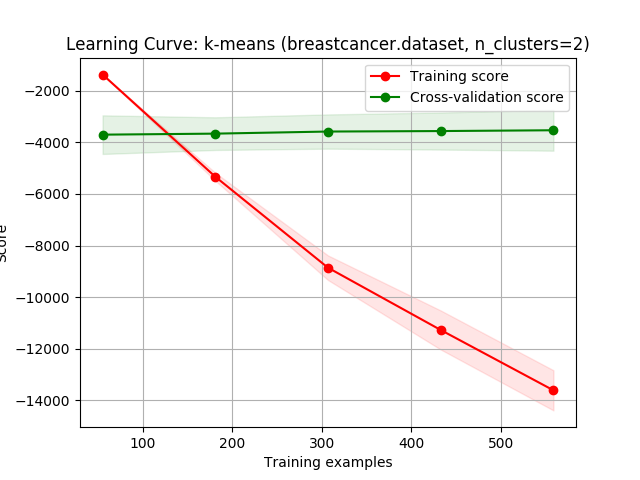
\includegraphics[width=\linewidth]{out/kmeans/cancer-learning.png}
            \caption{Learning curve, cancer.dataset}
            \label{fig:kmeans-learning-cancer}
          \end{subfigure}

        \caption{Learning curves for both data sets, using optimal parameters.}
        \label{fig:kmeans-learning}
        \end{figure}

        Both data sets seem to converge into clusters reasonably quickly, as shown by the low variance in the cross validation scores. Interestingly though, the variation in the car data set's cross validation score narrows as the proportion of training examples used approaches 100\%. The fit times of each test were recorded at 0.102s for the car data, and 0.044s for the cancer data. These running times will be compared to other algorithms and methods in a later section.

        Though the cancer data set is clustered better than the car data set by $k$-means, this same drop in variance is not observed. This suggests to me that the completeness of the instances in the car data had some effect on that outcome. However, this will be looked into further when dimensionality reduction algorithms are applied prior to clustering.

    \subsection{Expectation Maximization}
      The expectation maximization algorithm was tested using gaussian mixture models, with negative log-likelihood as the performance metric.

      \subsubsection{Parameter selection}
        Expectation maximization, in this implementation, takes one main parameter, which is the number of ``components''. Each algorithm was tested for best performance with between 1 and 15 components inclusive, as shown in \Fref{fig:em-comp}.

        \begin{figure}[htb]
        \centering

          \begin{subfigure}{0.5\textwidth}
            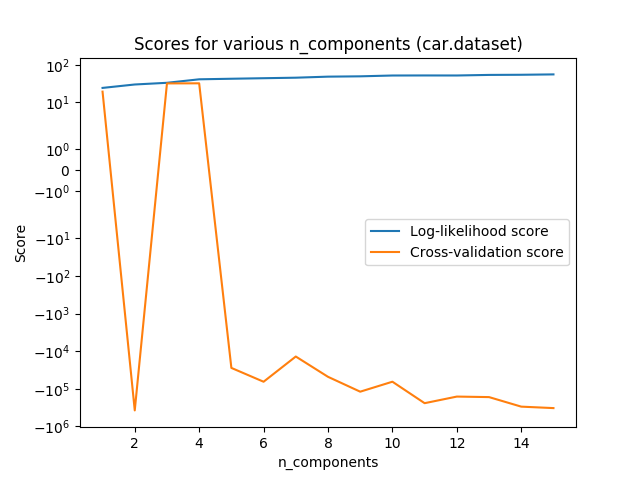
\includegraphics[width=\linewidth]{out/em/car-components-testing.png}
            \caption{Scores, car.dataset}
            \label{fig:em-comp-car}
          \end{subfigure}\hfil
          \begin{subfigure}{0.5\textwidth}
            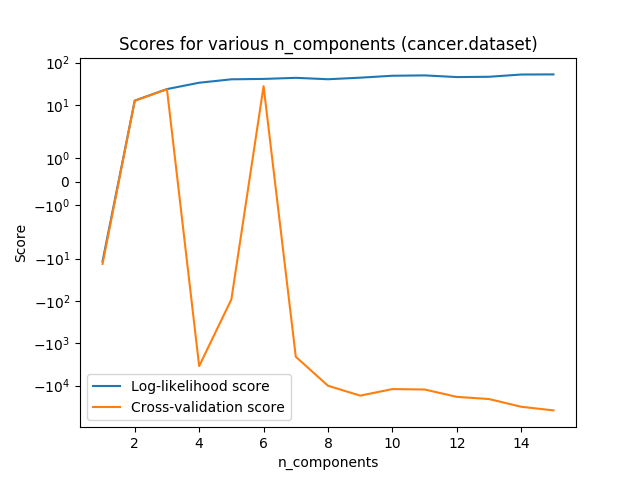
\includegraphics[width=\linewidth]{out/em/cancer-components-testing.png}
            \caption{Scores, cancer.dataset}
            \label{fig:em-comp-cancer}
          \end{subfigure}

        \caption{Log-likelihood of classifiers for both data sets with varying n\_components.}
        \label{fig:em-comp}
        \end{figure}

        In this case, the goal was to find the lowest number of components which resulted in the best scoring, as higher numbers of components increase running time. To satisfy this requirement, the car data set was chosen to have 4 components, while the cancer data set performed better with 3.

      \subsubsection{Performance}
        The learning curves for both data sets using expectation maximization are shown in \Fref{fig:em-learning}.

        \begin{figure}[htb]
        \centering

          \begin{subfigure}{0.5\textwidth}
            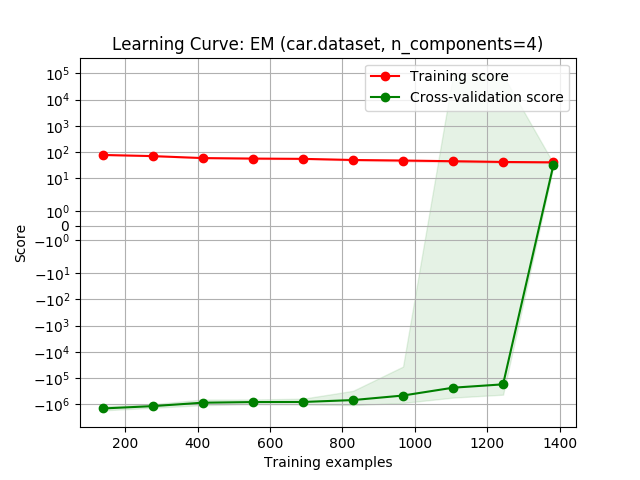
\includegraphics[width=\linewidth]{out/em/car-learning.png}
            \caption{Learning curve, car.dataset}
            \label{fig:em-learning-car}
          \end{subfigure}\hfil
          \begin{subfigure}{0.5\textwidth}
            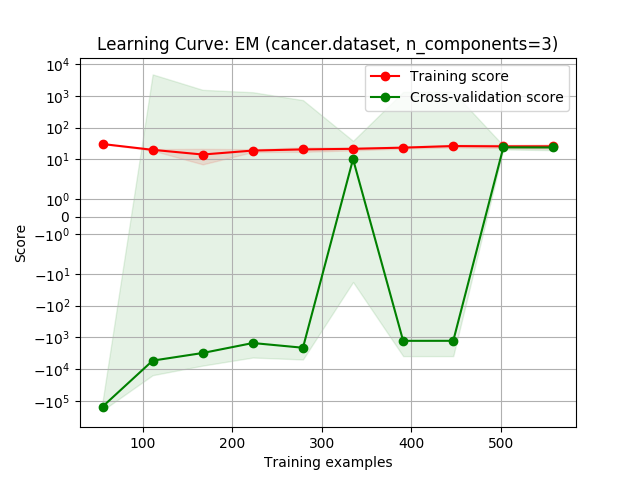
\includegraphics[width=\linewidth]{out/em/cancer-learning.png}
            \caption{Learning curve, cancer.dataset}
            \label{fig:em-learning-cancer}
          \end{subfigure}

        \caption{Learning curves for both data sets, using optimal parameters.}
        \label{fig:em-learning}
        \end{figure}

        The fit times for these classifiers were 0.025s for the car data, and 0.027s for the cancer data. Interestingly enough, both data sets have high variance in their cross validation scores at least at some point during training. In addition, the cancer data set seems to have had its cross-validation score converge with the training scores at the end of training. This result will be discussed further after attempting dimensionality reduction.

  \section{Dimensionality Reduction}
    We will now evaluate dimensionality reduction algorithms, which are used for feature selection and to consolidate high-dimension datasets into data more easily digestible by machine learning algorithms. Note that with higher numbers of components, the dimensionality of the algorithm outputs is too high for 2D or 3D visualizations to be sufficient. As such, we will evaluate much of the performance of each algorithm on how it assists a clustering algorithm or a neural network in the next sections. This section will focus on identifying which dimensionality reduction algorithms are effective in clustering the data alone. 

    \subsection{PCA}
      \Fref{fig:pca-plot} shows the best-found configuration for PCA to maximize clustering apparent on the first two feature spaces. Interestingly, the cancer data set did not have any variation in PCA dimensionality reduction across the first two features of the data set. Due to the high-dimensionality of PCA with larger numbers of components, it is difficult to show the effectiveness of the PCA algorithm at higher numbers of components.

      As such, the car data set showed the most apparently clustering on two features with 4 components, whereas the cancer data set did not show any change in clustering on the first two features after adding more components.

      \begin{figure}[htb]
      \centering

        \begin{subfigure}{0.5\textwidth}
          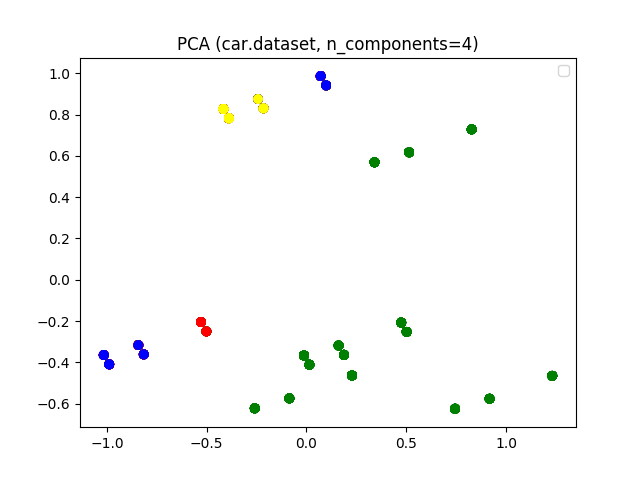
\includegraphics[width=\linewidth]{out/pca/car-pca-comp-4.png}
          \caption{PCA, car.dataset}
          \label{fig:pca-plot-car}
        \end{subfigure}\hfil
        \begin{subfigure}{0.5\textwidth}
          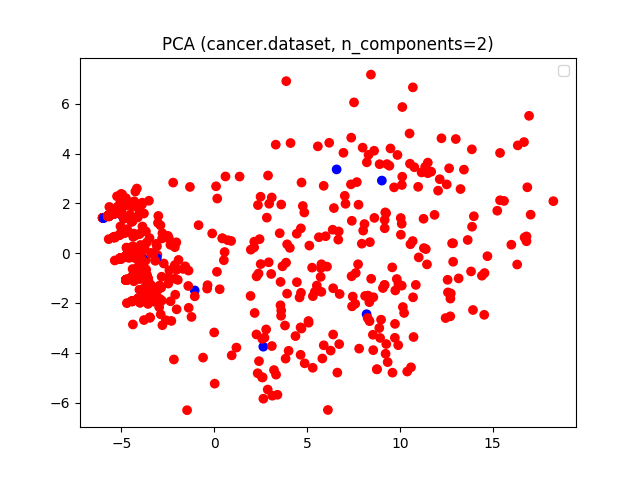
\includegraphics[width=\linewidth]{out/pca/cancer-pca-comp-2.png}
          \caption{PCA, cancer.dataset}
          \label{fig:pca-plot-cancer}
        \end{subfigure}

      \caption{PCA plots for both data sets.}
      \label{fig:pca-plot}
      \end{figure}

    \subsection{ICA}
      The ICA algorithm resulted in similar clustering to that of the PCA algorithm for the car data set, while clustering the cancer data into narrower bands that more effectively produced a cluster of blue points signifying the malignant tumor class. In this case, the number of components specified had a large effect on the plots of both data sets. The plots for the ICA algorithm can be seen in \Fref{fig:ica-plot}.

      \begin{figure}[htb]
      \centering

        \begin{subfigure}{0.5\textwidth}
          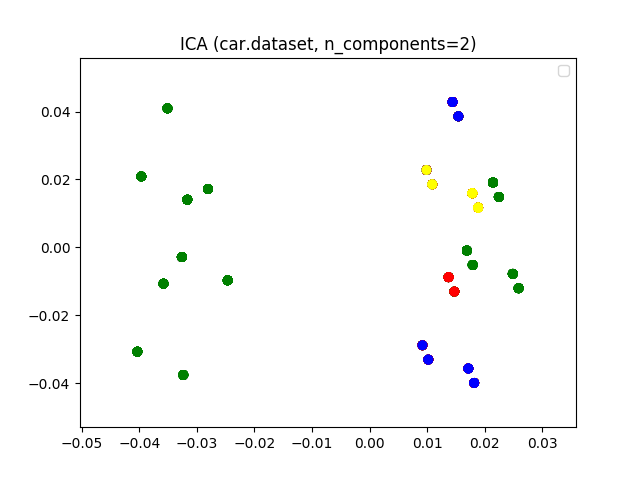
\includegraphics[width=\linewidth]{out/ica/car-ica-comp-2.png}
          \caption{ICA, car.dataset}
          \label{fig:ica-plot-car}
        \end{subfigure}\hfil
        \begin{subfigure}{0.5\textwidth}
          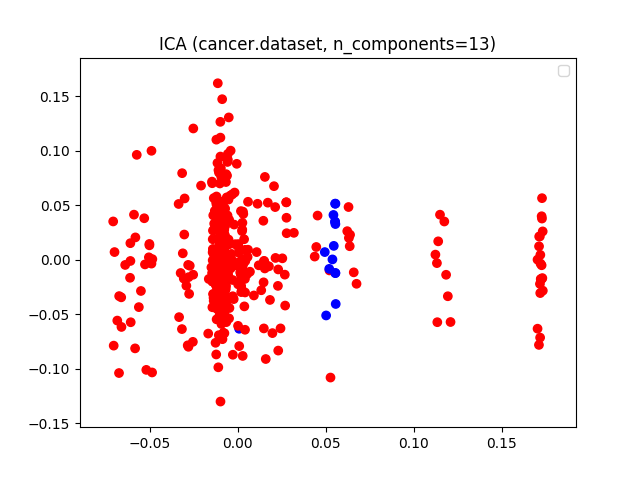
\includegraphics[width=\linewidth]{out/ica/cancer-ica-comp-13.png}
          \caption{ICA, cancer.dataset}
          \label{fig:ica-plot-cancer}
        \end{subfigure}

      \caption{ICA plots for both data sets.}
      \label{fig:ica-plot}
      \end{figure}

    \subsection{Randomized Projections}
      Unlike PCA and ICA, a run of randomized projections using the gaussian random projection algorithm from scikit-learn did not result in any meaningful clustering of either data set when plotted on two features, as shown in \Fref{fig:rp-plot}. The effectiveness of this algorithm on the data will be further evaluated when combined with another learner, such as a clustering algorithm or neural net.

      \begin{figure}[htb]
      \centering

        \begin{subfigure}{0.5\textwidth}
          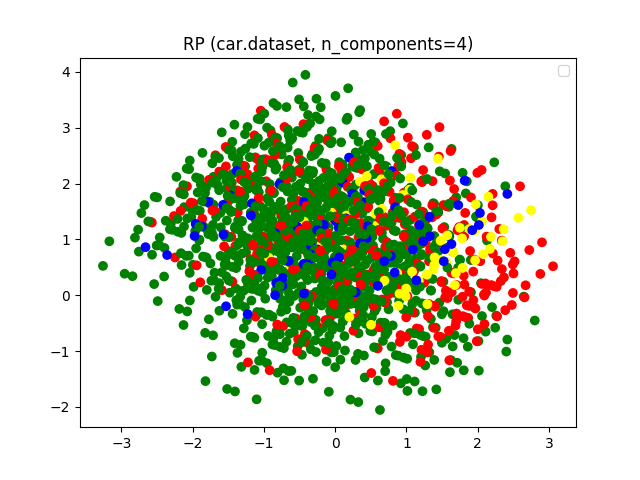
\includegraphics[width=\linewidth]{out/rp/car-rp-comp-4.png}
          \caption{RP, car.dataset}
          \label{fig:rp-plot-car}
        \end{subfigure}\hfil
        \begin{subfigure}{0.5\textwidth}
          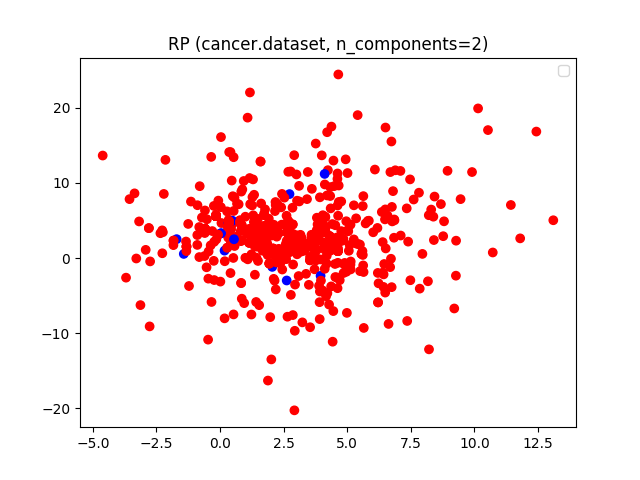
\includegraphics[width=\linewidth]{out/rp/cancer-rp-comp-2.png}
          \caption{RP, cancer.dataset}
          \label{fig:rp-plot-cancer}
        \end{subfigure}

      \caption{RP plots for both data sets.}
      \label{fig:rp-plot}
      \end{figure}

  \section{Clustering with Dimensionality Reduction}
    Both the $k$-means clustering algorithm and expectation maximization algorithms were run with ICA and PCA for dimensionality reduction and compared to the standard clustering runs without dimensionality reduction.

    \Fref{fig:cdr-plot-km-car} and \Fref{fig:cdr-plot-em-car} show the differences (or rather lack thereof) in the learning curves between the various runs with no dimensionality reduction, and with ICA and PCA. For the car dataset, dimensionality reduction had no discernible effect on the learning curve, further confirming the earlier hypothesis that such a complete covering of the attribute space does not gain any extra performance or information from reducing the dimensionality of the data.

    In addition, both randomized projection and feature agglomeration were used for further attempts at dimensionality reduction, however again no discernible difference was found.

    \begin{figure}[htb]
    \centering

      \begin{subfigure}{0.33\textwidth}
        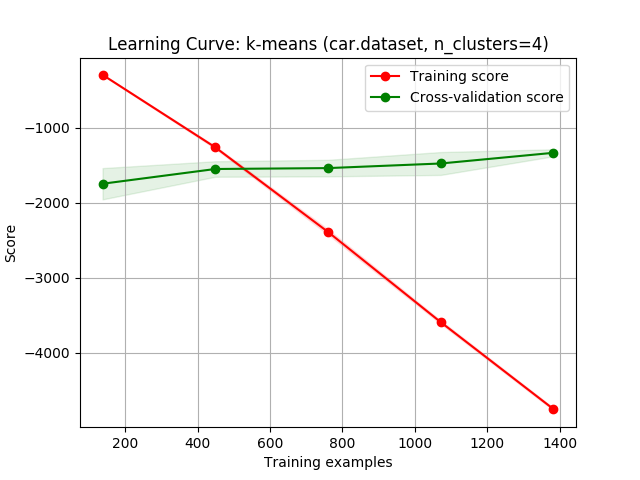
\includegraphics[width=\linewidth]{out/kmeans/car-learning.png}
        \caption{No DR, car.dataset}
      \end{subfigure}\hfil
      \begin{subfigure}{0.33\textwidth}
        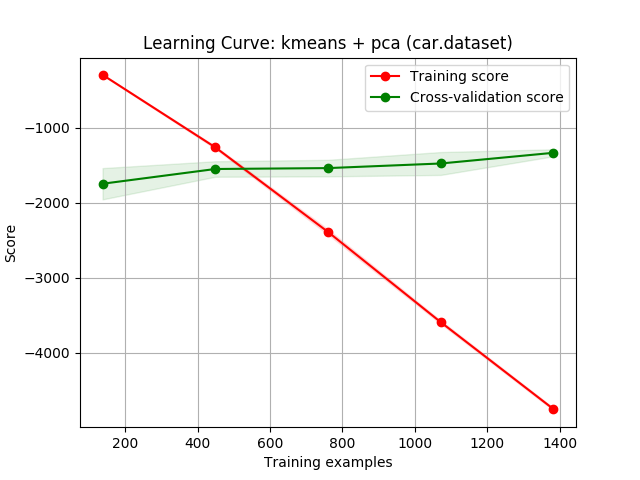
\includegraphics[width=\linewidth]{out/cluster_dr/car-kmeans-pca-learning.png}
        \caption{PCA, car.dataset}
      \end{subfigure}\hfil
      \begin{subfigure}{0.33\textwidth}
        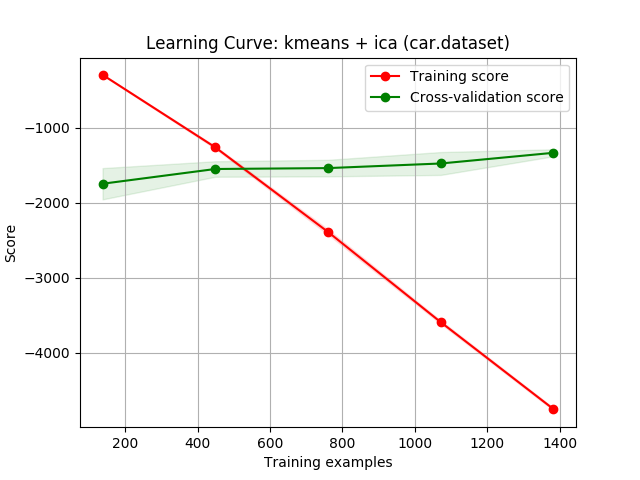
\includegraphics[width=\linewidth]{out/cluster_dr/car-kmeans-ica-learning.png}
        \caption{ICA, car.dataset}
      \end{subfigure}

    \caption{$k$-means clustering, car.dataset}
    \label{fig:cdr-plot-km-car}
    \end{figure}

    \begin{figure}[htb]
    \centering

      \begin{subfigure}{0.33\textwidth}
        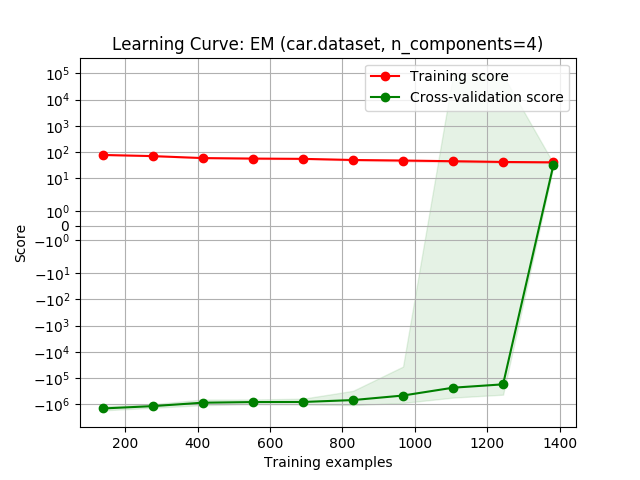
\includegraphics[width=\linewidth]{out/em/car-learning.png}
        \caption{No DR, car.dataset}
      \end{subfigure}\hfil
      \begin{subfigure}{0.33\textwidth}
        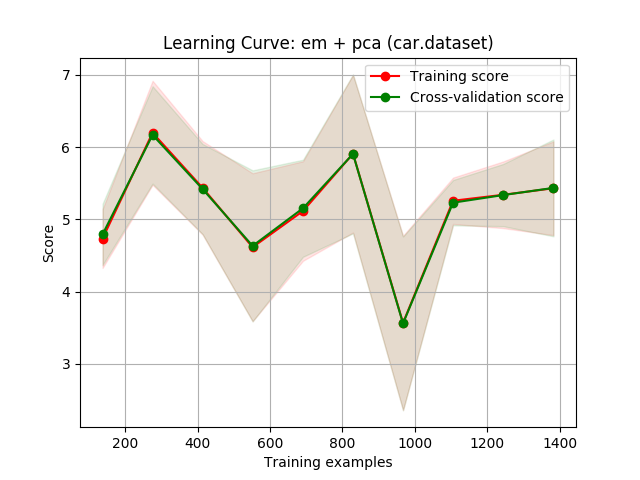
\includegraphics[width=\linewidth]{out/cluster_dr/car-em-pca-learning.png}
        \caption{PCA, car.dataset}
      \end{subfigure}\hfil
      \begin{subfigure}{0.33\textwidth}
        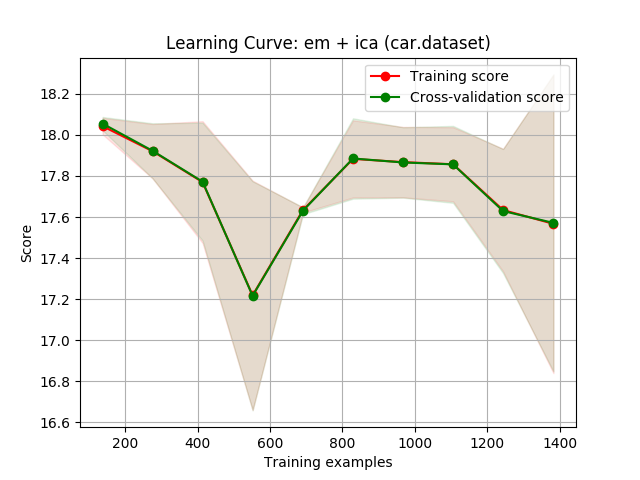
\includegraphics[width=\linewidth]{out/cluster_dr/car-em-ica-learning.png}
        \caption{ICA, car.dataset}
      \end{subfigure}

    \caption{Expectation maximization, car.dataset}
    \label{fig:cdr-plot-em-car}
    \end{figure}
    
    \Fref{fig:cdr-plot-km-cancer} and \Fref{fig:cdr-plot-em-cancer} show the same results for running clustering algorithms along with or without dimensionality reduction, however this time on the breast cancer data set. For the $k$-means clustering algorithm, the cross-validation score reported with dimensionality reduction was much lower than in the case of running clustering without DR. However, while running expectation maximization, the effects of using any form of dimensionality reduction are less pronounced.

    The resulting plot with $k$-means clustering and dimensionality reduction on the cancer data is indicative of DR having a positive effect on the clustering algorithm. Namely, it seems that using DR allowed the $k$-means clustering algorithm to filter out noise by grouping together attributes that have relationships.

    \begin{figure}[htb]
    \centering

      \begin{subfigure}{0.33\textwidth}
        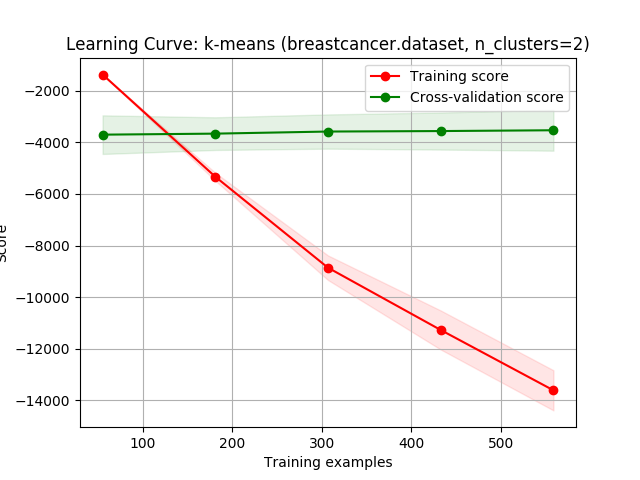
\includegraphics[width=\linewidth]{out/kmeans/cancer-learning.png}
        \caption{No DR, cancer.dataset}
      \end{subfigure}\hfil
      \begin{subfigure}{0.33\textwidth}
        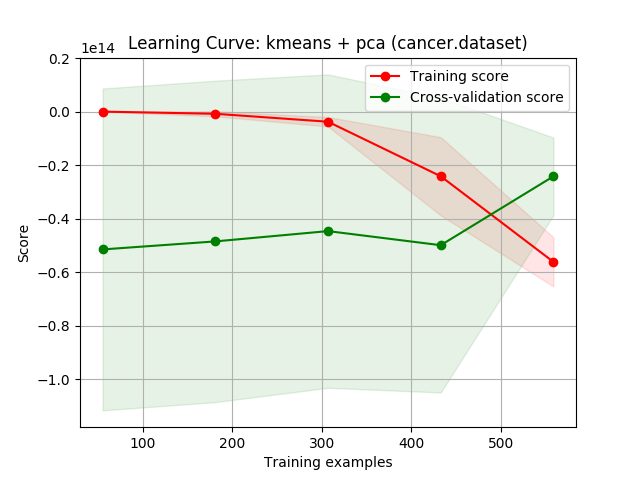
\includegraphics[width=\linewidth]{out/cluster_dr/cancer-kmeans-pca-learning.png}
        \caption{PCA, cancer.dataset}
      \end{subfigure}\hfil
      \begin{subfigure}{0.33\textwidth}
        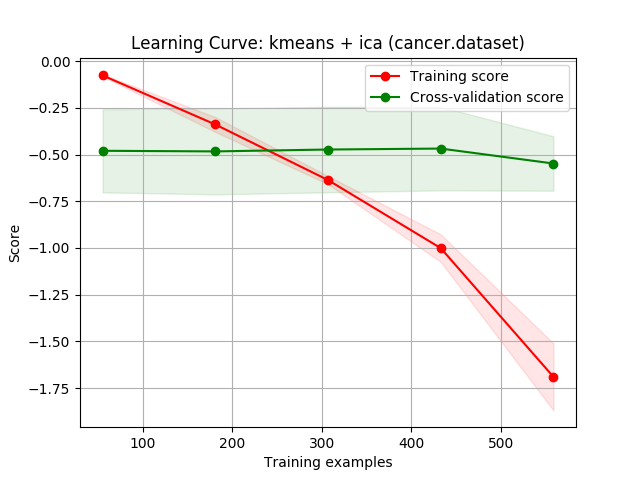
\includegraphics[width=\linewidth]{out/cluster_dr/cancer-kmeans-ica-learning.png}
        \caption{ICA, cancer.dataset}
      \end{subfigure} 

    \caption{$k$-means clustering, cancer.dataset}
    \label{fig:cdr-plot-km-cancer}
    \end{figure}


    \begin{figure}[htb]
    \centering

      \begin{subfigure}{0.33\textwidth}
        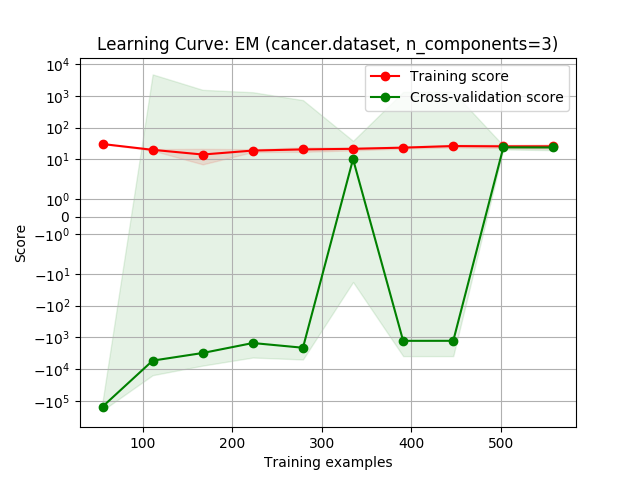
\includegraphics[width=\linewidth]{out/em/cancer-learning.png}
        \caption{No DR, cancer.dataset}
      \end{subfigure}\hfil
      \begin{subfigure}{0.33\textwidth}
        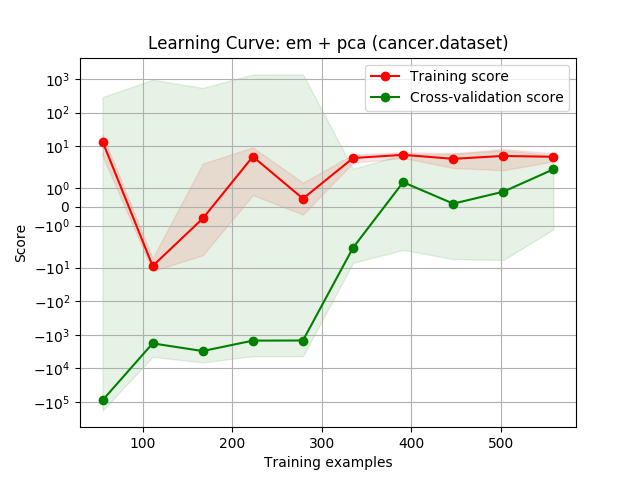
\includegraphics[width=\linewidth]{out/cluster_dr/cancer-em-pca-learning.png}
        \caption{PCA, cancer.dataset}
      \end{subfigure}\hfil
      \begin{subfigure}{0.33\textwidth}
        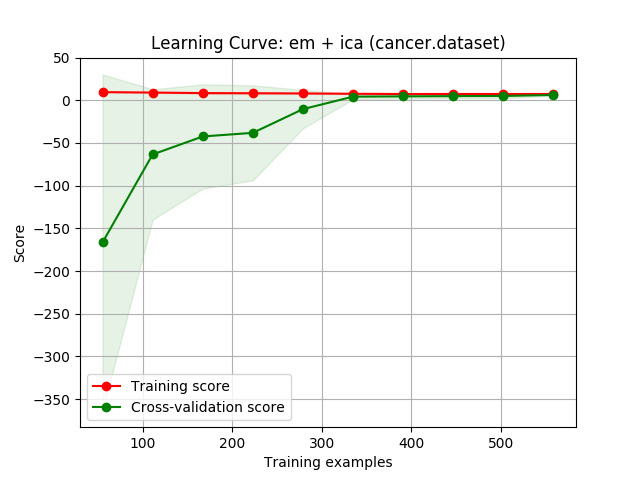
\includegraphics[width=\linewidth]{out/cluster_dr/cancer-em-ica-learning.png}
        \caption{ICA, cancer.dataset}
      \end{subfigure}

    \caption{Expectation maximization, cancer.dataset}
    \label{fig:cdr-plot-em-cancer}
    \end{figure}

  \section{Neural Networks with Dimensionality Reduction}
    Each data set was then reduced in dimensionality with the previously-discussed algorithms, and analyzed for overall score to evaluate if dimensionality reduction is appropriate for use in either data set. Both data sets used the adam solver provided by scikit-learn, along with a max iteration setting of 1000.

    \Fref{fig:nndr-plot-car} shows the results for the car data set. Again, per the prior hypothesis, dimensionality reduction did not have much to offer for the car data. All 3 runs with or without dimensionality reduction resulted in a cross-validation score somewhere around 0.8. Interestingly, the neural network trained with PCA-reduced data had the lowest running time at 1.716s, with no DR and ICA following at 3.659s and 4.275s respectively. However, despite the fact that PCA allowed the neural network to converge faster over 1000 iterations, the reduction of dimensionality for a complete set of data may not be desirable here in all cases.

    \begin{figure}[htb]
    \centering

      \begin{subfigure}{0.33\textwidth}
        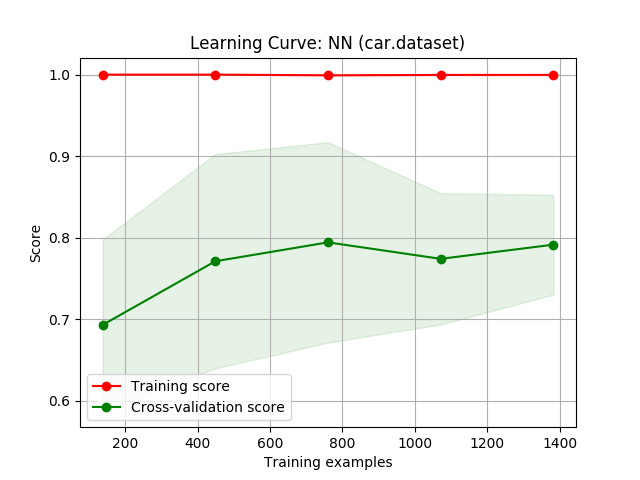
\includegraphics[width=\linewidth]{out/nn_dr/car-learning.png}
        \caption{No DR, car.dataset}
      \end{subfigure}\hfil
      \begin{subfigure}{0.33\textwidth}
        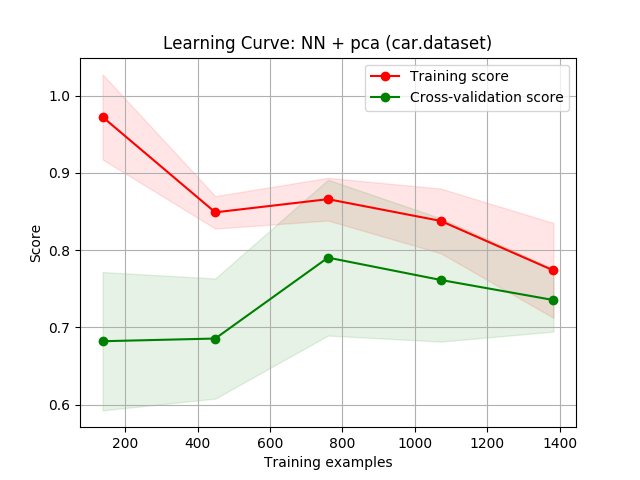
\includegraphics[width=\linewidth]{out/nn_dr/car-pca-learning.png}
        \caption{PCA, car.dataset}
      \end{subfigure}\hfil
      \begin{subfigure}{0.33\textwidth}
        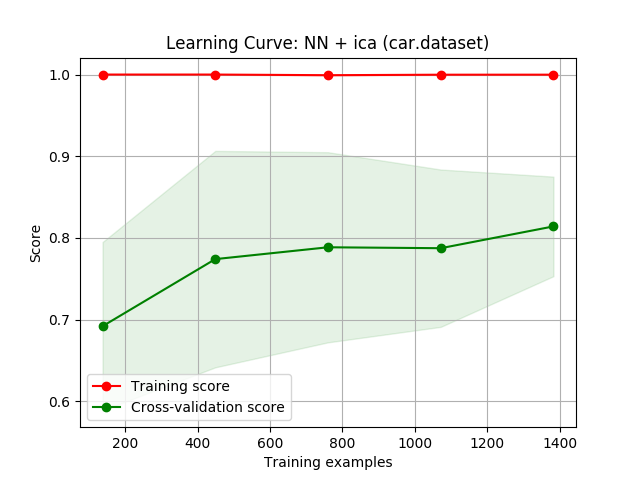
\includegraphics[width=\linewidth]{out/nn_dr/car-ica-learning.png}
        \caption{ICA, car.dataset}
      \end{subfigure}

    \caption{Neural network with and without dimensionality reduction, car.dataset}
    \label{fig:nndr-plot-car}
    \end{figure}

    \Fref{fig:nndr-plot-cancer} shows the results for the cancer data set. The effects of dimensionality reduction here are much more apparent. The training run using ICA for dimensionality reduction performed the best, converging to a cross-validation score of nearly 1.0 in around 100 less training examples than with PCA or no DR. However, the training time for ICA in this case was around 10x that of the alternatives, with a runtime of 0.352s as opposed to the running times of 0.048s and 0.038s for no DR and PCA respectively. 

    \begin{figure}[htb]
    \centering

      \begin{subfigure}{0.33\textwidth}
        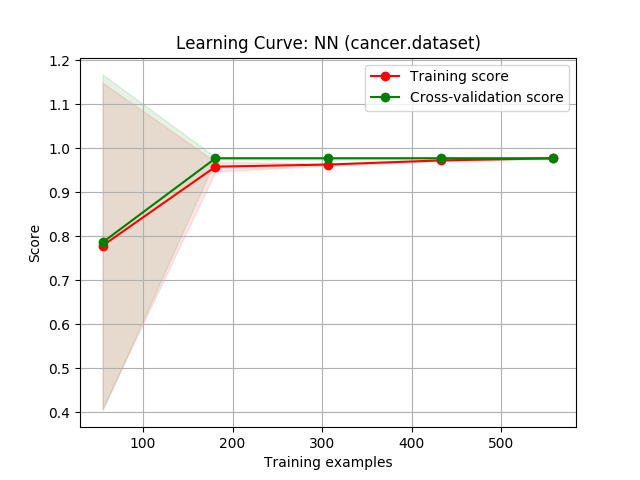
\includegraphics[width=\linewidth]{out/nn_dr/cancer-learning.png}
        \caption{No DR, cancer.dataset}
      \end{subfigure}\hfil
      \begin{subfigure}{0.33\textwidth}
        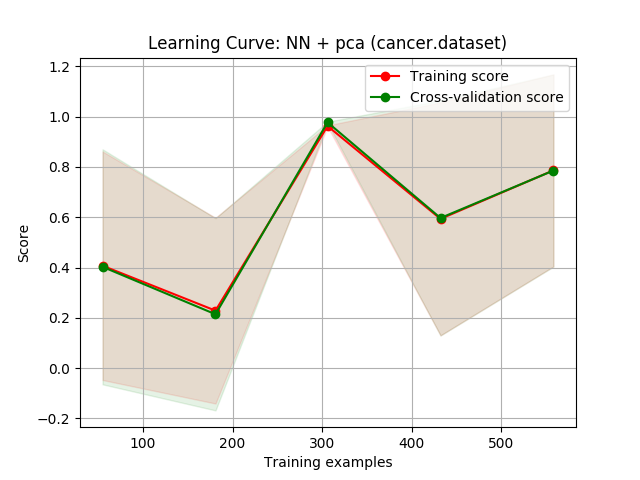
\includegraphics[width=\linewidth]{out/nn_dr/cancer-pca-learning.png}
        \caption{PCA, cancer.dataset}
      \end{subfigure}\hfil
      \begin{subfigure}{0.33\textwidth}
        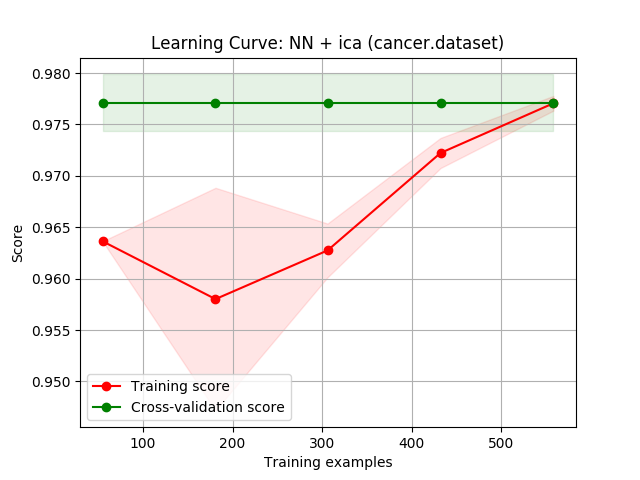
\includegraphics[width=\linewidth]{out/nn_dr/cancer-ica-learning.png}
        \caption{ICA, cancer.dataset}
      \end{subfigure}

    \caption{Neural network with and without dimensionality reduction, cancer.dataset}
    \label{fig:nndr-plot-cancer}
    \end{figure}

    From this information, one might conclude that due to the small attribute space presented by the car and cancer data sets, dimensionality reduction isn't as effective in reducing fit time on smaller dimensions of data. However, if the attribute space of our data was 100-dimensional, for example, we would see a considerable improvement by using dimensionality reduction to reduce the problem space first, as neural networks can be extremely slow on larger dimensional data.

  \section{Neural Networks with Clustering}
    Finally, we'll evaluate neural networks once more, this time using clustering algorithms in place of dimensionality reduction algorithms. As it was difficult to determine how to properly incorporate gaussian mixture models into this test using scikit-learn, only $k$-means clustering will be evaluated.

    \Fref{fig:nnc-plot-car} shows that using $k$-means clustering in conjunction with the car data set caused the overall accuracy of the neural network to drop. Because neural networks are a weight optimization problem, it would make sense that reducing the dimensionality of a complete data set using a clustering algorithm causes loss in all cases except where accuracy is 100\% for the clustering algorithm. Because this is not the case, the clustering algorithm causes the cross-validation score of the neural network to drop from just under 0.8 to under 0.6.

    The neural network without clustering did take longer to run, however, with a running time of 3.371s as opposed to 0.937s with clustering. But, because the accuracy fell so much by reducing dimensionality, there is no place in using clustering on the car data set in addition to a neural network, as they are already effectively doing the same job.

    \begin{figure}[htb]
    \centering

      \begin{subfigure}{0.5\textwidth}
        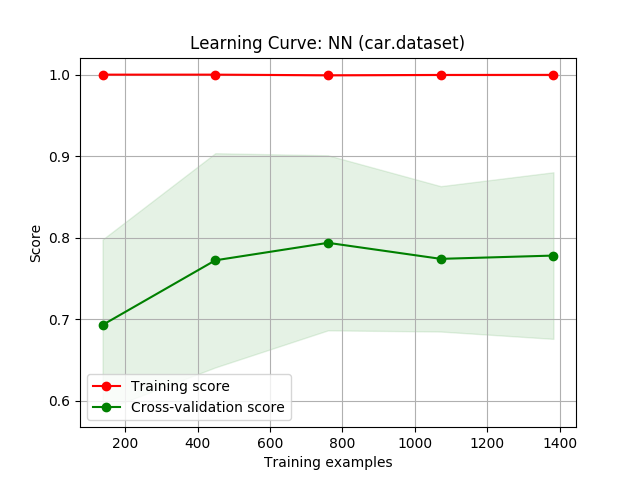
\includegraphics[width=\linewidth]{out/nn_cluster/car-learning.png}
        \caption{No clustering, car.dataset}
      \end{subfigure}\hfil
      \begin{subfigure}{0.5\textwidth}
        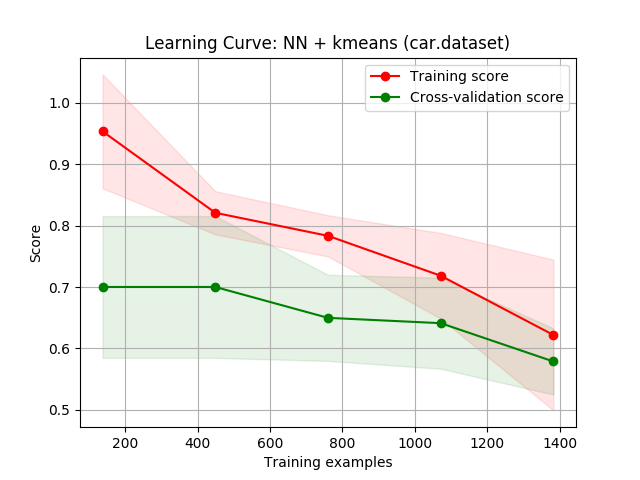
\includegraphics[width=\linewidth]{out/nn_cluster/car-kmeans-learning.png}
        \caption{$k$-means, car.dataset}
      \end{subfigure}

    \caption{Neural network with and without clustering, car.dataset}
    \label{fig:nnc-plot-car}
    \end{figure}

    \begin{figure}[htb]
    \centering

      \begin{subfigure}{0.5\textwidth}
        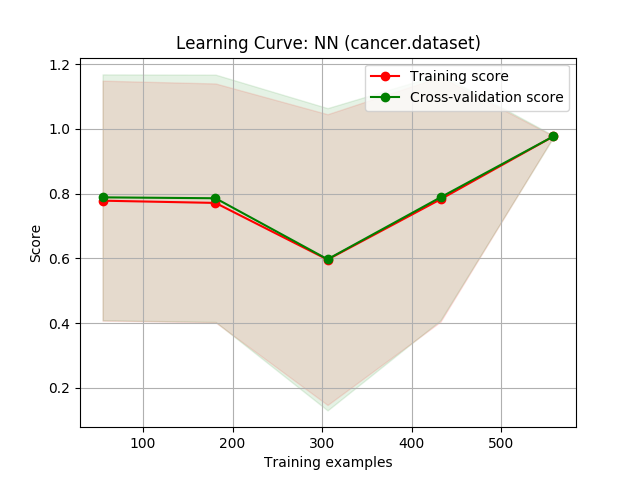
\includegraphics[width=\linewidth]{out/nn_cluster/cancer-learning.png}
        \caption{No clustering, cancer.dataset}
      \end{subfigure}\hfil
      \begin{subfigure}{0.5\textwidth}
        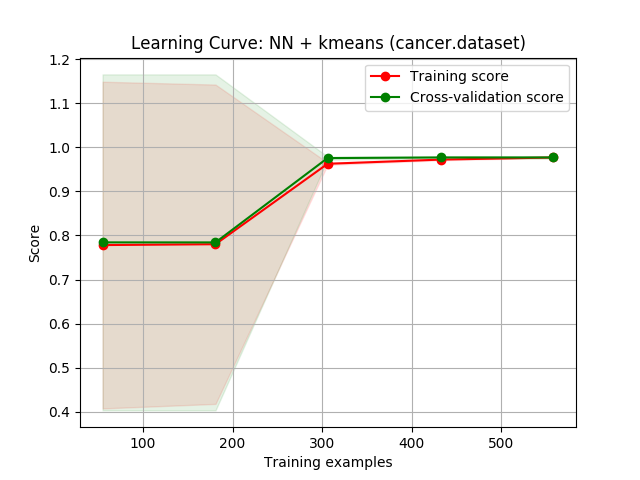
\includegraphics[width=\linewidth]{out/nn_cluster/cancer-kmeans-learning.png}
        \caption{$k$-means, cancer.dataset}
      \end{subfigure}

    \caption{Neural network with and without clustering, cancer.dataset}
    \label{fig:nnc-plot-cancer}
    \end{figure}

    \Fref{fig:nnc-plot-cancer} shows that clustering had the opposite effect with the cancer data set. Instead of dropping in accuracy, the addition of clustering as a feature to the input of the neural network resulted in faster convergence and better cross-validation scores at earlier iterations for the neural network using $k$-means clustering over the neural network without clustering. This shows an interesting interaction between the two algorithms. The cluster estimation provided to the neural network, if it is relatively accurate, can be weighted as an important feature for estimating the output for an unseen input. Therefore, if the clustering algorithm works well, the neural network will take less iterations to converge.

    The clustering algorithm also doesn't take much longer to run -- the neural network with $k$-means clustering trained in 0.055s, while the neural network without clustering took 0.040s to train. Thus, clustering the data first to concatenate an ``initial estimate'' is effective at converging the weights of the neural network over fewer examples and training iterations.

    In all, in addition to another learning algorithm, clustering can easily function as a dimensionality reduction algorithm in itself. However, with small attribute spaces as we've discussed prior in this report, concatenating clustering results to the initial input was chosen as the best fit (pun intended) for this part of the assignment.

  \section{Discussion}
    It is difficult to say whether clustering had tangible benefits over supervised learning or randomized optimization. Without better visualization of how the feature spaces within a data set interact, I was resigned to only looking at the clustering based on two features instead of the entire $n$-dimensional feature space of each data set.

    However, dimensionality reduction seemed relatively ineffective overall on both data sets because of the narrowness of the data. The car data set did not respond well to dimensionality reduction very well at all when applied to any other algorithms, for reasons mentioned earlier regarding completeness. There were performance improvements in some isolated cases, however it is difficult to give a recommendation for using these algorithms with these data sets without further, more granular investigation.

    We also saw that clustering algorithms present the opportunity to give a neural network a good starting point for weight optimization by starting with an uninformed (via unsupervised learning) guess based on the properties of the data. However, the main takeaway from this report is that dimensionality reduction and even clustering may not make sense for every type of data. For the two data sets I used, I had mixed results. The cancer data responded better to the addition of clustering or dimensionality reduction on top of an existing neural network, but both data sets lacked the width needed to postulate about the running time differences between running learning algorithms on a dimensionally reduced data set as opposed to an untouched one of high dimension.

  \section{Conclusion}
    In exploring this topic in the future, I'd look toward using data sets with higher dimensions and without complete attribute coverage in order to further test the efficacy of dimensionality reduction on both discrete and continuous data. In that case, I would expect clustering and/or dimensionality reductions to provide huge performance gains for large, wide data sets when combined with a neural network as we did in previous sections.


\end{document}